\chapter[Constructing IPFs for Medical Images: A Segmentation Problem]{Constructing IPFs for Medical Images:\\A Segmentation Problem}

%---
\section{Chapter Overview}

In Chapter~\ref{chap:ipfs}, the image partition forest (IPF) data structure was introduced, together with an accompanying set of algorithms. This chapter looks at how IPFs can be constructed from medical image slices (2D) or volumes (3D) by adapting the morphological watershed and waterfall algorithms \cite{beucher94,marcotegui05}. This forms the backdrop for Chapter~\ref{chap:featureid}, which describes IPF algorithms for performing automatic feature identification.

The IPF construction process described in the following sections uses the watershed algorithm to generate the lowest (leaf) layer of the IPF (the finest partition of the image). The waterfall algorithm is then used to generate the higher layers of the IPF: in particular, each non-leaf layer of the IPF is the result of running an iteration of the waterfall algorithm on the layer immediately below it.

%---
\section{The Watershed Transform}

\subsection{Overview}

The grey-scale watershed transform is an image segmentation algorithm which takes a grey-scale image (whether 2D or 3D) as input and produces a partition of that image into regions, one for each local minimum in the image. It does this by simulating a process of flooding that starts with a pool of water at each local minimum. As the algorithm proceeds, these pools grow, until some of them are on the point of touching each other. At this point, watersheds (dams) are added to keep the pools apart: in segmentation terms, these will become region boundaries, which in turn will yield a partition of the original image into regions associated with its local minima.

%---
\stufigex{height=8cm}{segmentation-watershed-landscapeanalogy.png}{The landscape analogy: Viewing a 2D image as a 3D terrain}{fig:segmentation-watershed-landscapeanalogy}{t}
%---

The process is most easily visualized in 2D. An image $I$ may be considered as a height map, or landscape, as shown in Figure~\ref{fig:segmentation-watershed-landscapeanalogy}: for every point $(x,y)$ in the domain of the image, there is an associated pixel value $I(x,y)$ which gives the height of the landscape at that point. In the 8-bit image shown, for instance, black pixels in the image correspond to a height of $0$ and white pixels correspond to a height of $255$. The watershed process involves metaphorically taking this surface, poking holes through its local minima and lowering it perpendicularly into a lake. As the water rises, the pools of water, or catchment basins, associated with the local minima grow (see Figure~\ref{fig:segmentation-watershed-construction}(a)). Eventually, these catchment basins will meet (Figure~\ref{fig:segmentation-watershed-construction}(b)) and a watershed will be constructed to keep them apart (Figure~\ref{fig:segmentation-watershed-construction}(c)). This process continues until the water has reached the top of the landscape, at which point the algorithm terminates. The watersheds generated during the process divide the landscape into the valleys associated with its local minima (see Figure~\ref{fig:segmentation-watershed-construction}(d)), which is equivalent to dividing the base image into regions.

%---
\begin{figure}[t]
\begin{center}
	\subfigure[Beginning the flooding]{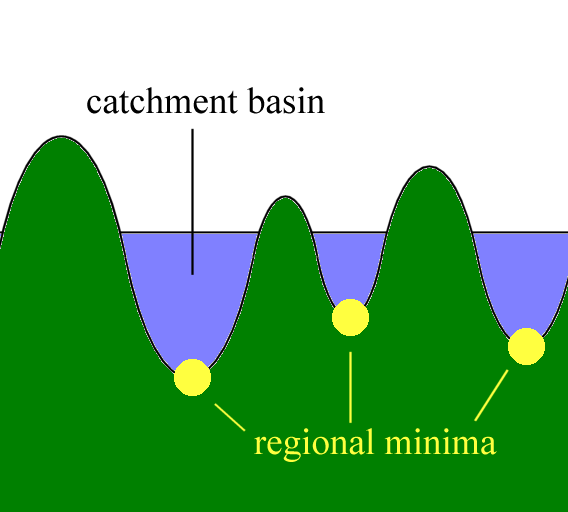
\includegraphics[height=6cm]{segmentation-watershed-construction1.png}}%
	\hspace{4mm}%
	\subfigure[Two catchment basins meet]{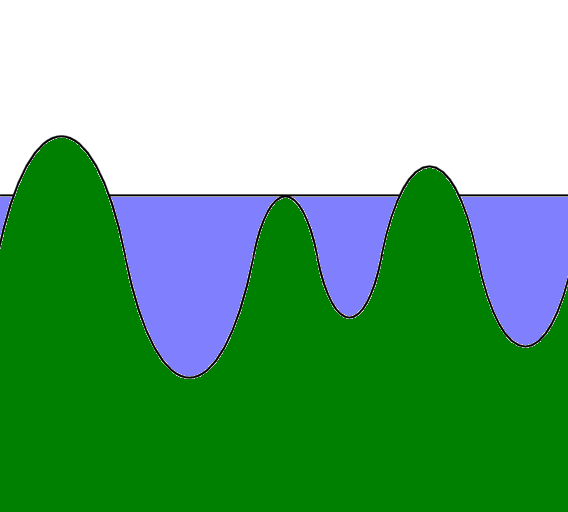
\includegraphics[height=6cm]{segmentation-watershed-construction2.png}}%
	\hspace{4mm}%
	\subfigure[Building a watershed at the join point]{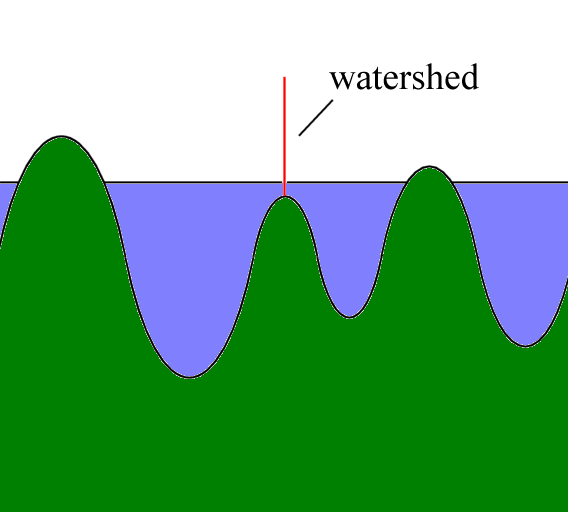
\includegraphics[height=6cm]{segmentation-watershed-construction3.png}}%
	\hspace{4mm}%
	\subfigure[The final division into regions]{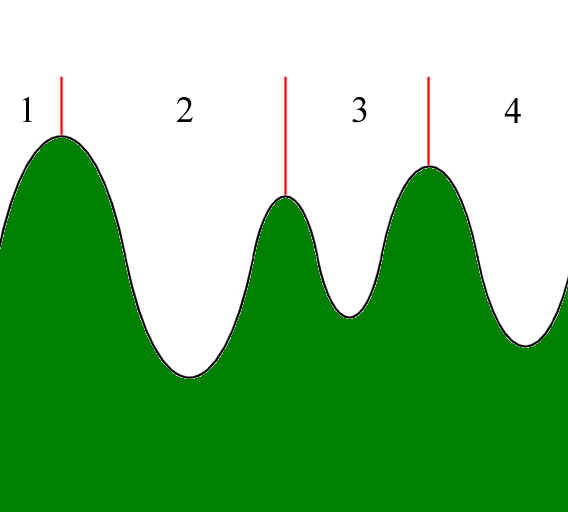
\includegraphics[height=6cm]{segmentation-watershed-construction4.png}}%
\end{center}
\caption{The watershed construction process}
\label{fig:segmentation-watershed-construction}
\end{figure}
%---

\subsection{Pre-Processing}

\subsubsection{Overview}

Using the watershed algorithm as just described to process an image will almost invariably have undesired results, for two reasons:
%
\begin{enumerate}
\item The watershed algorithm segments the landscape into its valleys, but there is no a priori reason to suppose that these valleys correspond to features of interest in the original image.
\item The image is unlikely to be smooth: it may have large numbers of local minima, especially in the presence of noise. In terrain terms, this is equivalent to having a pock-marked landscape, which the watershed algorithm will over-segment into far too many regions (each minor dimple in the landscape gets treated as a separate valley).
\end{enumerate}
%
The first problem is very domain-specific, depending on both the type of image being segmented and the particular features we are trying to segment. When trying to segment organs in abdominal CT scans, we observe that each organ exhibits a high degree of grey-value homogeneity: that is, the grey value varies relatively little across it. This implies that the image landscape is relatively flat over the area of each organ, or alternatively that the magnitude of the gradient is small there. By contrast, we hope that the gradient magnitude at the edges of organs will be relatively large (although in practice it is not always as large as we would like). The gradient magnitude of the original image is thus an image whose valleys are much more likely to correspond to organs than those of the original image (see Figure~\ref{?}): we can use this as the input to the watershed algorithm in place of our original input.

The second problem is much harder to solve: the solution lies partly in smoothing the original image (a pre-processing step), and partly in merging the large number of small regions generated by the watershed algorithm together into larger regions with more semantic meaning (a post-processing step for which we use the waterfall algorithm, described later). There are a number of different possible approaches to smoothing the image, a few of which are described in the following subsections.

\subsubsection{Gaussian Filtering}

Gaussian filtering (also called Gaussian blurring) is essentially a form of weighted pixel averaging based on a discrete approximation to the nD version of the Gaussian (normal) distribution (where n is the dimension of the image we're blurring). The 1D Gaussian is defined as:
%
\[
g_\sigma^1(x) = \frac{1}{\sigma\sqrt{2\pi}} \exp \frac{-x^2}{2\sigma^2}
\]
%
Its 2D version\footnote{The 3D version can be obtained analogously as $g_\sigma^3(x,y,z) = g_\sigma^1(x) \times g_\sigma^1(y) \times g_\sigma^1(z)$.} can be obtained by multiplying a 1-D Gaussian in the x direction with one in the y direction:
%
\[
g_\sigma^2(x,y) = g_\sigma^1(x) \times g_\sigma^1(y) = \frac{1}{2\pi\sigma^2} \exp \left( -\frac{x^2+y^2}{2\sigma^2} \right)
\]
%
The graph of the 1D Gaussian is the familiar bell curve; the 2D version is a bell-shaped surface (see Figure~\ref{fig:segmentation-watershed-gaussian2d}).

%---
\stufigex{height=8cm}{segmentation-watershed-gaussian2d.png}{The 2D Gaussian is a bell-shaped surface}{fig:segmentation-watershed-gaussian2d}{t}
%---

Using this for image blurring involves forming a symmetric mask (see Figure~\ref{fig:segmentation-watershed-gaussianmask}) from the values of $g_\sigma^2(x,y)$ at discrete points in a grid centred at the origin (e.g.~for a 3x3 mask, we should calculate $g_\sigma^2$ at $(-1,-1), (0,-1), (1,-1), \ldots, (0,0), \ldots, (1,1)$). The mask then needs to be normalized by dividing by the sum of all the values in it (this is done to ensure that regions of uniform intensity in the image will be unaffected by smoothing). This procedure can be used to generate masks of any size.

%---
\begin{figure}[t]
\begin{center}
\begin{tabular}{|c|c|c|}
\hline
0.0585 & 0.0965 & 0.0585 \\
\hline
0.0965 & 0.1592 & 0.0965 \\
\hline
0.0585 & 0.0965 & 0.0585 \\
\hline
\end{tabular}%
$\;\; \longrightarrow \;\;$%
\begin{tabular}{|c|c|c|}
\hline
0.0751 & 0.1238 & 0.0751 \\
\hline
0.1238 & 0.2042 & 0.1238 \\
\hline
0.0751 & 0.1238 & 0.0751 \\
\hline
\end{tabular}
\end{center}
\caption{As an example, we'll calculate a 3x3 mask for the 2D Gaussian $g_1^2(x,y)$ (i.e. the Gaussian with standard deviation $\sigma = 1$). First we calculate the values of $g_1^2(x,y)$ at the grid points (i.e. we calculate $g_1^2(-1,-1), \ldots, g_1^2(1,1)$) to give us the unnormalized mask (left); then, we normalize it by dividing through by the sum of all the values in the mask to give the final result (right).}
\label{fig:segmentation-watershed-gaussianmask}
\end{figure}
%---

The actual blurring is performed by \emph{convolving} an image $I$ with the mask to form a new image $I'$. Letting $M_\sigma^{3,3}$ be the 3x3 mask, this is written as $I' = I \otimes M_\sigma^{3,3}$. Convolution means overlaying the mask on each pixel of the image in turn, multiplying the value of each pixel in the mask by the value of the pixel beneath it, summing the results and using the value thus obtained as the value of the centre pixel in the blurred image. For the 3x3 mask with $\sigma = 1$, this means that:
%
\begin{eqnarray*}
I'(x,y)
& = & 0.0751 \times (I(x-1,y-1) + I(x+1,y-1) + I(x-1,y+1) + I(x+1,y+1)) \; + \\
&   & 0.1238 \times (I(x,y-1) + I(x,y+1) + I(x-1,y) + I(x+1,y)) \; + \\
&   & 0.2042 \times I(x,y)
\end{eqnarray*}
%
This begs the question of what happens when the mask is placed on one of the border pixels of the image (i.e.~such that part of it is outside the image). The simplest way to deal with this is to perform the weighted sum with the pixels that are in range, and then normalize by dividing by the sum of the mask values used. For instance, using this scheme we would have:
%
\[
I'(0,1) = \frac{0.0751 \times (I(1,0) + I(1,2)) + 0.1238 \times (I(0,0) + I(0,2) + I(1,1)) + 0.2042 \times I(0,1)}{2 \times 0.0751 + 3 \times 0.1238 + 0.2042}
\]
%
Gaussian filtering is very good at smoothing an image (see Figure~\ref{?}), but it isn't generally sufficient as the sole pre-processing filter for image segmentation because it uniformly blurs the image. This makes the image smoother, but if we smooth it enough to make it suitable for input to the watershed, we end up destroying fine detail in which we're interested (e.g.~boundaries betweens organs). For any application, this would cause problems; for medical applications, in particular, it is unacceptable. The solution is to be selective about how much blurring we do in different parts of the image: specifically, we want to blur a lot in areas of little or no interest, and blur a minimal amount (or not at all) near features of interest, such as edges between organs. Each of the following two approaches described aims to accomplish this.

% TODO: Figure here

\subsubsection{Spatially-Variant Gaussian Filtering}

Spatially-variant Gaussian filtering (SVGF) is a simple technique I developed to perform non-uniform Gaussian blurring. The essence of the idea is to use a Gaussian filter whose standard deviation varies with its location in the image. High standard deviations cause greater smoothing, whilst a filter with a low standard deviation smoothes less strongly. The key is to ensure that the filter has a high standard deviation away from suspected edges, and a low standard deviation when near to them. This requires two things: an estimate of where the interesting edges in the image lie (obviously we don't know where they are exactly: this is effectively what we're trying to determine when segmenting the image) and a mapping from the edge estimate image to the space of standard deviations (i.e.~$\mathbb{R}^+$). The gradient magnitude of the original image (after initial smoothing with a simple Gaussian filter as described above) provides a suitable edge estimate, but the mapping requires a bit more thought.

A suitable mapping function must map high values in the edge estimate image (representing the higher estimated likelihood of an edge at that location) to a low standard deviation (thus avoiding blurring the edges) and low values to a high standard deviation (thus maximising the blurring away from the edges). In practice, we want to avoid blurring if the edge estimate for a pixel is anything other than negligible: there needs to be a sharp falloff as the edge estimate for a pixel gets bigger, so a linear decrease in $\sigma$ values won't suffice (see Figure~\ref{?}).

% TODO: Figure here

This still gives us a wide choice of mapping functions, but experiments showed that a sigmoid function works well in practice. For example, consider an 8-bit edge estimate image whose values range from $0$ (minimal likelihood of an edge) to $255$ (maximal likelihood). The canonical sigmoid function is given by:
%
\[
y = \frac{1}{1 + e^{-x}}
\]
%
We want to transform it into a sigmoid function which starts high at $x = 0$ and rapidly drops off to a low level. To do this, we start by deciding on the points on the shape of the normal sigmoid curve to which we want $f_1 = 0$ and $f_2 = 255$ to map (for example, mapping $f_1$ to $x_1 = 6$ and $f_2$ to $x_2 = -100$ works well in this case). We then decide on the maximum and minimum values $y_h$ and $y_\ell$ we wish our sigmoid curve to take (here, $y_h = 8$ and $y_\ell = 0$ are sensible values). Finally, we calculate the required function as follows:
%
\begin{eqnarray*}
s_x & = & (f_2 - f_1)/(x_2 - x_1) \\
o_x & = & f_1/s_x - x_1 \\
s_y & = & y_h - y_\ell \\
o_y & = & y_\ell \\
y & = & s_y/(1 + \exp(-x/s_x + o_x)) + o_y
\end{eqnarray*}
%
A suitable mapping function for the 8-bit edge estimate image is thus
%
\[
y = \frac{8}{1 + \exp(106x/255 - 6)},
\]
%
a function which starts off at nearly $8$ when $x = 0$, then drops off rapidly to nearly zero at around $x = 30$ (see Figure~\ref{fig:segmentation-watershed-sigmoid}).

%---
\stufigex{height=10cm}{segmentation-watershed-sigmoid.png}{An example sigmoid function that maps the edge estimate at a pixel to the standard deviation of the Gaussian filter to apply there}{fig:segmentation-watershed-sigmoid}{t}
%---

SVGF produces good results when used in combination with normal Gaussian filtering: in particular, performing a small amount of Gaussian filtering followed by running the image through the spatially-variant filter works well. This is described further in \textbf{Constructing the Pre-Processing Pipeline}, below.

\subsubsection{Anisotropic Diffusion Filtering}

Anisotropic diffusion filtering (ADF) is a standard technique for doing edge-preserving smoothing on an image, originally introduced by Perona and Malik in \cite{perona90}. The idea comes from the fact that solving a heat equation of the form
%
\[
\pd{I(x,y,t)}{t} = \nabla^2 I(x,y,t) \equiv \nabla \cdot \nabla I(x,y,t)
\]
%
on an image $I_0(x,y)$, by setting $I(x,y,0) = I_0(x,y)$ as the initial condition, is equivalent to convolving $I_0$ with a Gaussian of standard deviation $\sqrt{2t}$. (In other words, by finding the solution to the heat equation at a time $t_0$, we are effectively blurring the image with the corresponding Gaussian.) Perona and Malik's idea was that by replacing $\nabla I(x,y,t)$ in the equation with $C \nabla I(x,y,t)$, for some $C$, the results of solving the heat equation could be influenced to depend on where we expect the edges in the original image to be. In particular, if we assume that the gradient magnitude of the original image provides a reasonable estimate of where the edges are, then we can write $C = c(|\nabla I(x,y,t)|)$, for some function $c$, giving us the anisotropic diffusion equation
%
\[
\pd{I(x,y,t)}{t} = \nabla \cdot c(|\nabla I(x,y,t)|) \nabla I(x,y,t).
\]
%
We thereby introduce a prior expectation of where the edges to be into the equation, allowing us to influence the smoothing process so as to preserve them. The key to this is in how we specify $c$. We want the image to be blurred less where $|\nabla I|$ is large, so $c$ must yield a small value for large $|\nabla I|$ and a larger value for small $|\nabla I|$. There are obviously an infinite number of functions which would satisfy this, but an effective $c$ from the literature (and, in particular, the one used in the Insight Toolkit \cite{ITK} implementation I used) is given by
%
\[
c(|\nabla I|) = e^{-\frac{|\nabla I|^2}{2k^2}},
\]
%
where $k$ is simply a parameter used to affect the extent to which smoothing is affected by the gradient magnitude image.

ADF thus takes two parameters: a time $t_0$, which indirectly specifies the standard deviation of the Gaussian used, and $k$, as just mentioned. It is significantly more effective than SVGF in practice, so I now use it in preference to SVGF.

\subsubsection{Constructing the Pre-Processing Pipeline}

TODO

\iffalse

\subsection{Definitions}

Formally, an image is considered to be a function $f: \Omega_{\subset \mathbb{Z}^n} \to \mathbb{Z}$ that maps elements of the domain $\Omega$ to integer grey values. (For instance, a $2$-dimensional $512 \times 512$ image could be defined to have domain $\Omega = \{(x,y) : 0 \le x,y < 512\}$.) A pixel $\mathbf{p} \in \Omega$ is defined to have height $f(\mathbf{p})$ and neighbour set $N(\mathbf{p})$, according to some implementation-defined notion of neighbourhood: usually neighbourhood is defined so that pixels are either 4- or 8-connected in 2D, and 6- or 26-connected in 3D (see Figure~\ref{?}).

% TODO: Figure here

A \smgidx[singular minimum]{singular minimum} of an image is a point whose neighbours are all strictly higher than it. Formally, $\mathbf{p}$ is a singular minimum iff $\forall \mathbf{p'} \in N(\mathbf{p}) \cdot f(\mathbf{p'} > f(\mathbf{p})$. A \smgidx[plateau]{plateau} of an image is a maximal set of two or more connected pixels of equal altitude. A \smgidx[plateau!minimal]{minimal plateau} is a plateau from which it is impossible to descend, and a \smgidx[plateau!non-minimal]{non-minimal plateau} is the opposite. Together, the singular minima and minimal plateaux of an image form the \smgidx[local minimum!of image]{local minima} of the image.

TODO

\fi

\subsection{Implementing the Watershed Transform}

Having described how the input image is pre-processed, we turn our attentions to the implementation of the watershed transform itself. We must first define a few terms, however. Formally, an image is considered to be a function $f: \Omega_{\subset \mathbb{Z}^n} \to \mathbb{Z}$ that maps elements of the domain $\Omega$ to integer grey values. (For instance, a $2$-dimensional $512 \times 512$ image could be defined to have domain $\Omega = \{(x,y) : 0 \le x,y < 512\}$.) A pixel $\mathbf{p} \in \Omega$ is defined to have height $f(\mathbf{p})$ and neighbour set $N(\mathbf{p})$, according to some implementation-defined notion of neighbourhood: usually neighbourhood is defined so that pixels are either 4- or 8-connected in 2D, and 6- or 26-connected in 3D (see Figure~\ref{?}).

% TODO: Figure here

A \smgidx[singular minimum]{singular minimum} of an image is a point whose neighbours are all strictly higher than it. Formally, $\mathbf{p}$ is a singular minimum iff $\forall \mathbf{p'} \in N(\mathbf{p}) \cdot f(\mathbf{p'}) > f(\mathbf{p})$. A \smgidx[plateau]{plateau} of an image is a maximal set of two or more connected pixels of equal altitude. A \smgidx[plateau!minimal]{minimal plateau} is a plateau from which it is impossible to descend, and a \smgidx[plateau!non-minimal]{non-minimal plateau} is the opposite. Together, the singular minima and minimal plateaux of an image form the \smgidx[local minimum!of image]{local minima} of the image.

\subsubsection{The Rainfalling Method}

There are two main approaches to implementing the watershed: the flooding, or immersion, method (see \cite{?} for an example), which works essentially as outlined in the overview above, or the rainfalling method, which is the approach I used in my implementation. The end results are equivalent (although there are implementation choices involved that can lead to subtle differences, depending on the precise algorithm chosen); the only fundamental difference is one of perspective.

The rainfalling method involves thinking of the valleys in the landscape as catchment basins. For each point on the landscape, we can picture what would happen if we dropped water on it from above: since water takes a path of least resistance, it will run downhill to a local minimum (the bottom of a valley) via a path of steepest descent (in the image, this corresponds to a path where each step involves moving to a lowest neighbour of the current point). The catchment basin of a particular local minimum can thus be viewed as all the points from which a path of steepest descent leads to the minimum in question. Evidently something has been left of this description, since a given point may have more than one path of steepest descent, leading to different local minima (see Figure~\ref{?}): in this case, any consistent (i.e.~not random) choice of which path to choose is sufficient.

% TODO: Figure here

\subsubsection{Dealing with Non-Minimal Plateaux}

Non-minimal plateaux cause problems for the watershed transform, since it is unclear which way the water would run off them. There are various different approaches to dealing with this (e.g.~\cite{?,?,?}); the approach I took in practice was that in \cite{meijster98}, which involves transforming the image into one with no non-minimal plateaux (known as a lower-complete image).

In essence, the idea is to raise all plateau pixels up by their distance from the plateau edge (see Figure~\ref{?}). Of course, doing this naively doesn't work, since we might end up changing the ordering of the plateau pixels with respect to the other pixels in the image (see Figure~\ref{?}). The solution is to find the maximum amount by which we're going to raise a plateau pixel and multiply the base image by that before raising any pixels on the plateau: this has the effect of spreading the landscape heights out to accommodate the new altitudes in the middle (see Figure~\ref{?}).

% TODO: Figures here

Implementing this is relatively straightforward using a queue (see Listing~\ref{?}). The basic idea is to add all pixels with a lower neighbour to the queue at the start, then gradually flood out from them a level at a time (essentially a breadth-first search), incrementing the distance counter after each level.

\subsubsection{Fletching}

Given the lower-complete image constructed in the previous section, the next step is to calculate paths of steepest descent for each point in the image. Evidently the na\"ive approach of finding a steepest path for each point in turn would be computationally costly, but this is unnecessary as the problem of finding the steepest paths exhibits optimal substructure. Our approach, then, is to construct an arrow on each pixel (hence the process being called fletching) which indicates the first step of the steepest path from that pixel (see Figure~\ref{?}). In the case of a local minimum, the arrow is a self-loop back to the pixel itself (for a minimal plateau, one of the pixels is chosen as a canonical element of the plateau and all the other pixels point to it); for all other pixels, the arrow points to a lowest neighbouring node.

The implementation (see Listing~\ref{?}) uses Tarjan's disjoint-set forest data structure (see Appendix~\ref{?}). The idea is to combine all the minimum points into their respective local minima using this data structure, and make all the other non-minimal points point to one of their lower neighbours. We also take the opportunity to numerically label all the canonical points during this phase of the process.

% TODO: Figure here

\subsubsection{Labelling the Image}

TODO

%---
\section{The Waterfall Algorithm}

TODO
